% Auto-generated by the analysis pipeline — do not edit
% y > 0: Underreacts  |  y < 0: Overreacts
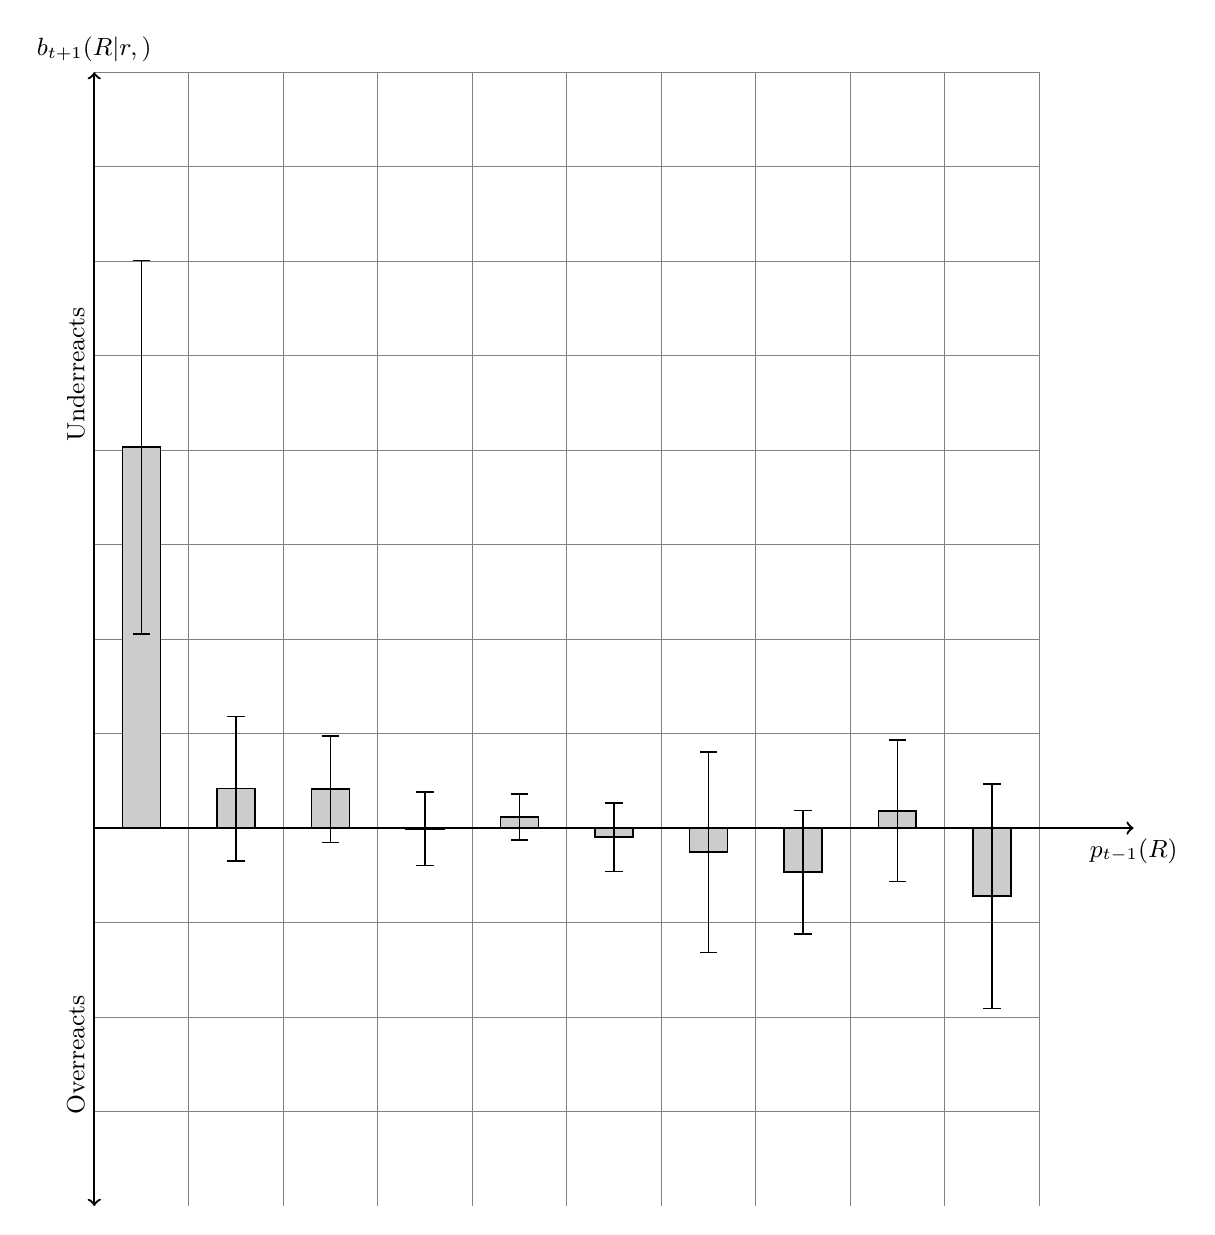
\begin{tikzpicture}[scale=12]
\draw[help lines,step=0.1] (0,-0.4) grid (1,0.8);
\filldraw[opaque,white!80!black] (0.03,0) rectangle (0.07,0.4031);
\draw[line width=0.6] (0.03,0) rectangle (0.07,0.4031);
\draw[line width=0.6,|-|] (0.05,0.2047) -- (0.05,0.6015);
\filldraw[opaque,white!80!black] (0.13,0) rectangle (0.17,0.0417);
\draw[line width=0.6] (0.13,0) rectangle (0.17,0.0417);
\draw[line width=0.6,|-|] (0.15,-0.0355) -- (0.15,0.1188);
\filldraw[opaque,white!80!black] (0.23,0) rectangle (0.27,0.0412);
\draw[line width=0.6] (0.23,0) rectangle (0.27,0.0412);
\draw[line width=0.6,|-|] (0.25,-0.0163) -- (0.25,0.0986);
\filldraw[opaque,white!80!black] (0.33,0) rectangle (0.37,-0.0008);
\draw[line width=0.6] (0.33,0) rectangle (0.37,-0.0008);
\draw[line width=0.6,|-|] (0.35,-0.0405) -- (0.35,0.0388);
\filldraw[opaque,white!80!black] (0.43,0) rectangle (0.47,0.0117);
\draw[line width=0.6] (0.43,0) rectangle (0.47,0.0117);
\draw[line width=0.6,|-|] (0.45,-0.0134) -- (0.45,0.0369);
\filldraw[opaque,white!80!black] (0.53,0) rectangle (0.57,-0.0097);
\draw[line width=0.6] (0.53,0) rectangle (0.57,-0.0097);
\draw[line width=0.6,|-|] (0.55,-0.0468) -- (0.55,0.0275);
\filldraw[opaque,white!80!black] (0.63,0) rectangle (0.67,-0.0255);
\draw[line width=0.6] (0.63,0) rectangle (0.67,-0.0255);
\draw[line width=0.6,|-|] (0.65,-0.1325) -- (0.65,0.0816);
\filldraw[opaque,white!80!black] (0.73,0) rectangle (0.77,-0.0468);
\draw[line width=0.6] (0.73,0) rectangle (0.77,-0.0468);
\draw[line width=0.6,|-|] (0.75,-0.1133) -- (0.75,0.0196);
\filldraw[opaque,white!80!black] (0.83,0) rectangle (0.87,0.0183);
\draw[line width=0.6] (0.83,0) rectangle (0.87,0.0183);
\draw[line width=0.6,|-|] (0.85,-0.0576) -- (0.85,0.0943);
\filldraw[opaque,white!80!black] (0.93,0) rectangle (0.97,-0.0722);
\draw[line width=0.6] (0.93,0) rectangle (0.97,-0.0722);
\draw[line width=0.6,|-|] (0.95,-0.1918) -- (0.95,0.0473);
\draw[line width=0.8,->]  (0,0) -- (1.1,0) node[below] {\small{$p_{t-1}(R)$}};
\draw[line width=0.8,<->] (0,-0.4) -- (0,0.8) node[above] {\small{$b_{t+1}(R|r,\xmark)$}};
\draw (0,0.48) node[above,rotate=90] {\small{Underreacts}};
\draw (0,-0.24) node[above,rotate=90] {\small{Overreacts}};
% ADD THEORY CURVE BELOW
\end{tikzpicture}
